\documentclass[8pt]{beamer}

% Beamer style
%\usetheme[secheader]{Madrid}
% \usetheme{CambridgeUS}
\useoutertheme{infolines}
\usecolortheme[rgb={0.65,0.15,0.25}]{structure}
% \usefonttheme[onlymath]{serif}
\beamertemplatenavigationsymbolsempty
%\AtBeginSubsection

% Packages
%\usepackage[french]{babel}
\usepackage[latin1]{inputenc}
\usepackage{color}
% \usepackage[dvipsnames]{xcolor}
\usepackage{xspace}
\usepackage{dsfont, stmaryrd}
\usepackage{amsmath, amsfonts, amssymb, stmaryrd, mathabx}
\usepackage{epsfig}
\usepackage{tikz}
\usepackage{url}
% \usepackage{ulem}
\usepackage{/home/robin/LATEX/Biblio/astats}
%\usepackage[all]{xy}
\usepackage{graphicx}

% Maths
% \newtheorem{theorem}{Theorem}
% \newtheorem{definition}{Definition}
\newtheorem{proposition}{Proposition}
% \newtheorem{assumption}{Assumption}
% \newtheorem{algorithm}{Algorithm}
% \newtheorem{lemma}{Lemma}
% \newtheorem{remark}{Remark}
% \newtheorem{exercise}{Exercise}
% \newcommand{\propname}{Prop.}
% \newcommand{\proof}{\noindent{\sl Proof:}\quad}
% \newcommand{\eproof}{$\blacksquare$}

% \setcounter{secnumdepth}{3}
% \setcounter{tocdepth}{3}
\newcommand{\pref}[1]{\ref{#1} p.\pageref{#1}}
\newcommand{\qref}[1]{\eqref{#1} p.\pageref{#1}}

% Colors : http://latexcolor.com/
\definecolor{darkred}{rgb}{0.65,0.15,0.25}
\definecolor{darkgreen}{rgb}{0,0.4,0}
\definecolor{darkred}{rgb}{0.65,0.15,0.25}
\definecolor{amethyst}{rgb}{0.6, 0.4, 0.8}
\definecolor{asparagus}{rgb}{0.53, 0.66, 0.42}
\definecolor{applegreen}{rgb}{0.55, 0.71, 0.0}
\definecolor{awesome}{rgb}{1.0, 0.13, 0.32}
\definecolor{blue-green}{rgb}{0.0, 0.87, 0.87}
\definecolor{red-ggplot}{rgb}{0.52, 0.25, 0.23}
\definecolor{green-ggplot}{rgb}{0.42, 0.58, 0.00}
\definecolor{purple-ggplot}{rgb}{0.34, 0.21, 0.44}
\definecolor{blue-ggplot}{rgb}{0.00, 0.49, 0.51}

% Commands
\newcommand{\backupbegin}{
   \newcounter{finalframe}
   \setcounter{finalframe}{\value{framenumber}}
}
\newcommand{\backupend}{
   \setcounter{framenumber}{\value{finalframe}}
}
\newcommand{\emphase}[1]{\textcolor{darkred}{#1}}
\newcommand{\comment}[1]{\textcolor{gray}{#1}}
\newcommand{\paragraph}[1]{\textcolor{darkred}{#1}}
\newcommand{\refer}[1]{{\small{\textcolor{gray}{{\cite{#1}}}}}}
\newcommand{\Refer}[1]{{\small{\textcolor{gray}{{[#1]}}}}}
\newcommand{\goto}[1]{{\small{\textcolor{blue}{[\#\ref{#1}]}}}}
\renewcommand{\newblock}{}

\newcommand{\tabequation}[1]{{\medskip \centerline{#1} \medskip}}
% \renewcommand{\binom}[2]{{\left(\begin{array}{c} #1 \\ #2 \end{array}\right)}}

% Variables 
\newcommand{\Abf}{{\bf A}}
\newcommand{\Beta}{\text{B}}
\newcommand{\Bcal}{\mathcal{B}}
\newcommand{\Bias}{\xspace\mathbb B}
\newcommand{\Cor}{{\mathbb C}\text{or}}
\newcommand{\Cov}{{\mathbb C}\text{ov}}
\newcommand{\cl}{\text{\it c}\ell}
\newcommand{\Ccal}{\mathcal{C}}
\newcommand{\cst}{\text{cst}}
\newcommand{\Dcal}{\mathcal{D}}
\newcommand{\Ecal}{\mathcal{E}}
\newcommand{\Esp}{\xspace\mathbb E}
\newcommand{\Espt}{\widetilde{\Esp}}
\newcommand{\Covt}{\widetilde{\Cov}}
\newcommand{\Ibb}{\mathbb I}
\newcommand{\Fcal}{\mathcal{F}}
\newcommand{\Gcal}{\mathcal{G}}
\newcommand{\Gam}{\mathcal{G}\text{am}}
\newcommand{\Hcal}{\mathcal{H}}
\newcommand{\Jcal}{\mathcal{J}}
\newcommand{\Lcal}{\mathcal{L}}
\newcommand{\Mt}{\widetilde{M}}
\newcommand{\mt}{\widetilde{m}}
\newcommand{\Nbb}{\mathbb{N}}
\newcommand{\Mcal}{\mathcal{M}}
\newcommand{\Ncal}{\mathcal{N}}
\newcommand{\Ocal}{\mathcal{O}}
\newcommand{\pt}{\widetilde{p}}
\newcommand{\Pt}{\widetilde{P}}
\newcommand{\Pbb}{\mathbb{P}}
\newcommand{\Pcal}{\mathcal{P}}
\newcommand{\Qcal}{\mathcal{Q}}
\newcommand{\qt}{\widetilde{q}}
\newcommand{\Rbb}{\mathbb{R}}
\newcommand{\Sbb}{\mathbb{S}}
\newcommand{\Scal}{\mathcal{S}}
\newcommand{\st}{\widetilde{s}}
\newcommand{\St}{\widetilde{S}}
\newcommand{\Tcal}{\mathcal{T}}
\newcommand{\todo}{\textcolor{red}{TO DO}}
\newcommand{\Ucal}{\mathcal{U}}
\newcommand{\Un}{\math{1}}
\newcommand{\Vcal}{\mathcal{V}}
\newcommand{\Var}{\mathbb V}
\newcommand{\Vart}{\widetilde{\Var}}
\newcommand{\Zcal}{\mathcal{Z}}

% Symboles & notations
\newcommand\independent{\protect\mathpalette{\protect\independenT}{\perp}}\def\independenT#1#2{\mathrel{\rlap{$#1#2$}\mkern2mu{#1#2}}} 
\renewcommand{\d}{\text{\xspace d}}
\newcommand{\gv}{\mid}
\newcommand{\ggv}{\, \| \, }
% \newcommand{\diag}{\text{diag}}
\newcommand{\card}[1]{\text{card}\left(#1\right)}
\newcommand{\trace}[1]{\text{tr}\left(#1\right)}
\newcommand{\matr}[1]{\boldsymbol{#1}}
\newcommand{\matrbf}[1]{\mathbf{#1}}
\newcommand{\vect}[1]{\matr{#1}} %% un peu inutile
\newcommand{\vectbf}[1]{\matrbf{#1}} %% un peu inutile
\newcommand{\trans}{\intercal}
\newcommand{\transpose}[1]{\matr{#1}^\trans}
\newcommand{\crossprod}[2]{\transpose{#1} \matr{#2}}
\newcommand{\tcrossprod}[2]{\matr{#1} \transpose{#2}}
\newcommand{\matprod}[2]{\matr{#1} \matr{#2}}
\DeclareMathOperator*{\argmin}{arg\,min}
\DeclareMathOperator*{\argmax}{arg\,max}
\DeclareMathOperator{\sign}{sign}
\DeclareMathOperator{\tr}{tr}
\newcommand{\ra}{\emphase{$\rightarrow$} \xspace}

% Hadamard, Kronecker and vec operators
\DeclareMathOperator{\Diag}{Diag} % matrix diagonal
\DeclareMathOperator{\diag}{diag} % vector diagonal
\DeclareMathOperator{\mtov}{vec} % matrix to vector
\newcommand{\kro}{\otimes} % Kronecker product
\newcommand{\had}{\odot}   % Hadamard product

% TikZ
\newcommand{\nodesize}{2em}
\newcommand{\edgeunit}{2.5*\nodesize}
\newcommand{\edgewidth}{1pt}
\tikzstyle{node}=[draw, circle, fill=black, minimum width=.75\nodesize, inner sep=0]
\tikzstyle{square}=[rectangle, draw]
\tikzstyle{param}=[draw, rectangle, fill=gray!50, minimum width=\nodesize, minimum height=\nodesize, inner sep=0]
\tikzstyle{hidden}=[draw, circle, fill=gray!50, minimum width=\nodesize, inner sep=0]
\tikzstyle{hiddenred}=[draw, circle, color=red, fill=gray!50, minimum width=\nodesize, inner sep=0]
\tikzstyle{observed}=[draw, circle, minimum width=\nodesize, inner sep=0]
\tikzstyle{observedred}=[draw, circle, minimum width=\nodesize, color=red, inner sep=0]
\tikzstyle{eliminated}=[draw, circle, minimum width=\nodesize, color=gray!50, inner sep=0]
\tikzstyle{empty}=[draw, circle, minimum width=\nodesize, color=white, inner sep=0]
\tikzstyle{blank}=[color=white]
\tikzstyle{nocircle}=[minimum width=\nodesize, inner sep=0]

\tikzstyle{edge}=[-, line width=\edgewidth]
\tikzstyle{edgebendleft}=[-, >=latex, line width=\edgewidth, bend left]
\tikzstyle{edgebendright}=[-, >=latex, line width=\edgewidth, bend right]
\tikzstyle{lightedge}=[-, line width=\edgewidth, color=gray!50]
\tikzstyle{lightedgebendleft}=[-, >=latex, line width=\edgewidth, bend left, color=gray!50]
\tikzstyle{lightedgebendright}=[-, >=latex, line width=\edgewidth, bend right, color=gray!50]
\tikzstyle{edgered}=[-, line width=\edgewidth, color=red]
\tikzstyle{edgebendleftred}=[-, >=latex, line width=\edgewidth, bend left, color=red]
\tikzstyle{edgebendrightred}=[-, >=latex, line width=\edgewidth, bend right, color=red]

\tikzstyle{arrow}=[->, >=latex, line width=\edgewidth]
\tikzstyle{arrowbendleft}=[->, >=latex, line width=\edgewidth, bend left]
\tikzstyle{arrowbendright}=[->, >=latex, line width=\edgewidth, bend right]
\tikzstyle{arrowred}=[->, >=latex, line width=\edgewidth, color=red]
\tikzstyle{arrowbendleftred}=[->, >=latex, line width=\edgewidth, bend left, color=red]
\tikzstyle{arrowbendrightred}=[->, >=latex, line width=\edgewidth, bend right, color=red]
\tikzstyle{arrowblue}=[->, >=latex, line width=\edgewidth, color=blue]
\tikzstyle{dashedarrow}=[->, >=latex, dashed, line width=\edgewidth]
\tikzstyle{dashededge}=[-, >=latex, dashed, line width=\edgewidth]
\tikzstyle{dashededgebendleft}=[-, >=latex, dashed, line width=\edgewidth, bend left]
\tikzstyle{lightarrow}=[->, >=latex, line width=\edgewidth, color=gray!50]

\newcommand{\dN}{\Delta N}
\newcommand{\dtau}{\Delta \tau}

% Directory
\newcommand{\figcp}{/home/robin/RECHERCHE/RUPTURES/EXPOSES/FIGURES}
\newcommand{\figDLR}{/home/robin/Bureau/Hawkes/segHP/article/StatComp2023/Revision/figures}

%====================================================================
%====================================================================

%====================================================================
%====================================================================
\begin{document}
%====================================================================
%====================================================================

%====================================================================
\title[Change-point in Poisson process]{Change-point detection in a Poisson process}

\author[S. Robin]{S. Robin \\ \medskip
joint work with E. Lebarbier, C. Dion-Blanc \refer{DLR23}}

\institute[]{Sorbonne universit�}

\date[LMO'24]{Laboratoire de math�matique d'Orsay, Feb. 2024}

%====================================================================
%====================================================================
\maketitle

%====================================================================
%====================================================================
\section*{Introduction}
%====================================================================
\frame{\frametitle{Examples} 

  \begin{tabular}{cc}
    \hspace{-.04\textwidth}
    \begin{tabular}{p{.45\textwidth}}
      \onslide+<2->{
      \paragraph{Point process on $t \in [0, 1]$.} \\ ~\\
      Event times:
      $$
      0 < T_1 < \dots T_i < \dots T_n < 1
      $$ \\
      
      Counting process:
      $$
      N(t) = \sum_{i=1}^n \Ibb\{T_i \leq t\}
      $$}      
      
      \onslide+<3->{
      \bigskip
      \paragraph{Poisson Process.}
      $$
      \{N(t)\}_{0 \leq t \leq 1} \sim PP(\lambda(t))
      $$}
    \end{tabular}
    & 
    \hspace{-.05\textwidth}
    \begin{tabular}{p{.5\textwidth}}
      \begin{overprint}
        \onslide<1>
        \paragraph{Bat cries} (night of the 17 jul. 2019) \\ ~\\
        \includegraphics[width=.45\textwidth, trim=0 10 10 10, clip=]{\figcp/ChauveSouris-GrandBourg}
        \onslide<2->
        \paragraph{Bat cries} (night of the 17 jul. 2019)\footnote{source: Vigie-Chiro program, Y. Bas, CESCO-MNHN} \\ 
        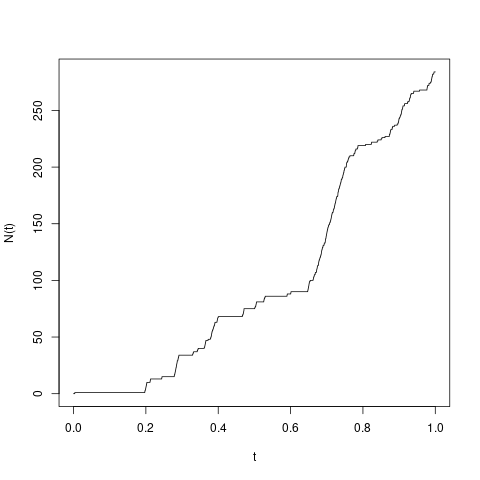
\includegraphics[width=.45\textwidth]{\figcp/FigSegPP-Chiroptere-seq2295-day2019-07-17-Path}
      \end{overprint}
    \end{tabular}
  \end{tabular}

  \bigskip
  \onslide+<3->{\paragraph{Intensity function $\lambda(t)$:} 
  $$
  \lambda(t) = \lim_{\Delta t \rightarrow 0} \frac{\Pbb\{N(t+\Delta t) - N(t) = 1\}}{\Delta t}, 
  \qquad \qquad 
  \Esp N(s) - \Esp N(t) = \int_t^s \lambda(u) \d u
  $$}
}

%====================================================================
\frame{\frametitle{Change-point detection} 

  \begin{tabular}{cc}
    \hspace{-.04\textwidth}
    \begin{tabular}{p{.45\textwidth}}
      \paragraph{Piecewise constant intensity function.} \\ ~ \\
      Change-points
      $$
      (\tau_0 =) \; 0 < \tau_1 \dots < \tau_{K-1} < 1 \; (= \tau_K)
      $$ \\
      
      For $t \in I_k = ]\tau_{k-1}, \tau_k]$:
      $$
      \lambda(t) = \lambda_k
      $$ 
      
      \bigskip 
      \ra Continuous piecewise linear cumulated intensity function   
      $$
      \Lambda(0, t) = \int_0^t \lambda(s) \d s.
      $$
    \end{tabular}
    & 
    \hspace{-.05\textwidth}
    \begin{tabular}{p{.45\textwidth}}
      \begin{overprint}
        \onslide<1>
        \paragraph{Bat cries} (night of the 17 jul. 2019)\footnote{source: Vigie-Chiro program, Y. Bas, CESCO-MNHN} \\
        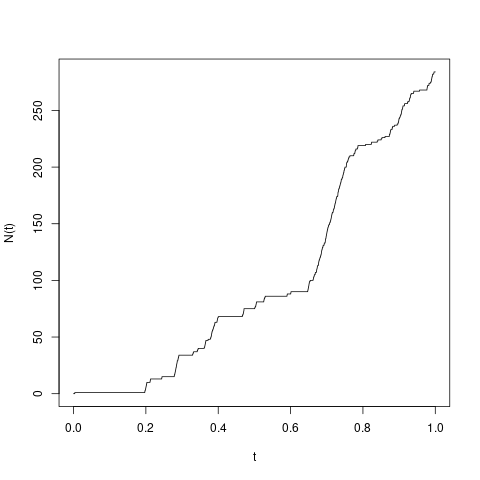
\includegraphics[width=.45\textwidth, trim=0 10 0 10, clip=]{\figcp/FigSegPP-Chiroptere-seq2295-day2019-07-17-Path}
        \onslide<2>
        \paragraph{Bat cries} (night of the 17 jul. 2019)\footnote{source: Vigie-Chiro program, Y. Bas, CESCO-MNHN} \\
        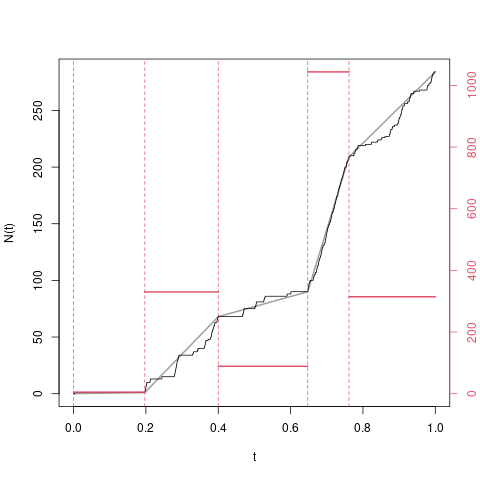
\includegraphics[width=.45\textwidth, trim=0 10 0 10, clip=]{\figcp/FigSegPP-Chiroptere-seq2295-day2019-07-17-Seg}
        \onslide<3>
        \paragraph{Kilauea eruptions} \\ ~ \\
        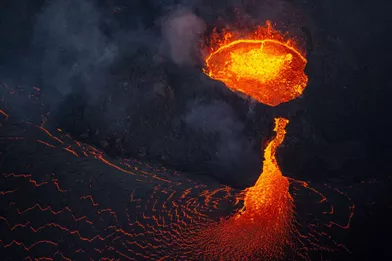
\includegraphics[width=.45\textwidth, height=.5\textheight]{\figcp/Kilauea-Wikipedia}
        \onslide<4>
        \paragraph{Kilauea eruptions} (from 1750 to 1984)\footnote{source: \refer{HoB17}} \\
        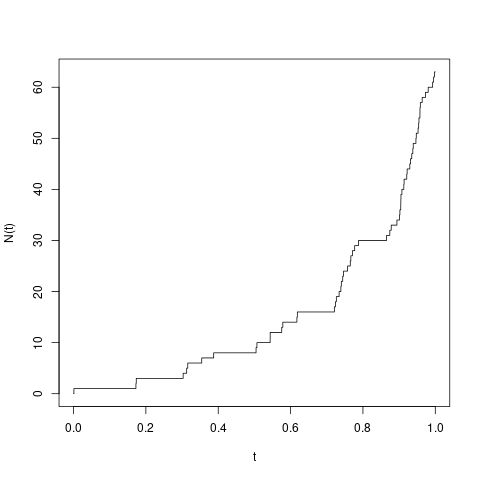
\includegraphics[width=.45\textwidth, trim=0 10 0 10, clip=]{\figcp/FigSegPP-Kilauea-Path}
        \onslide<5>
        \paragraph{Kilauea eruptions} (from 1750 to 1984)\footnote{source: \refer{HoB17}}  \\
        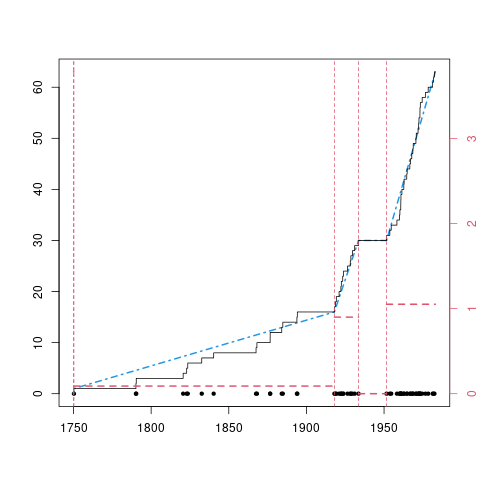
\includegraphics[width=.45\textwidth, trim=0 10 0 10, clip=]{\figcp/DLR23-ArXiv-Fig6a}
      \end{overprint}
    \end{tabular}
  \end{tabular}
  
  \bigskip \pause
  \paragraph{Aim.} 
  \begin{itemize}
   \item Segmentation: estimate $(\tau, \lambda)$ in a reasonnably fast manner
   \item Model selection: choose $K$
  \end{itemize}
}

%====================================================================
\frame{\frametitle{Change-point detection} 

  \paragraph{Three typical steps.}
  \begin{enumerate}
    \setlength{\itemsep}{1\baselineskip}
    \item Propose a set of reasonably realistic models;
    \item Design an (efficient) algorithm to get the parameter estimates;
    \item Choose among the models.
  \end{enumerate}

  \bigskip \bigskip \pause
  \paragraph{Example.}
  \begin{enumerate}
    \setlength{\itemsep}{1.25\baselineskip}
    \item $N(t)$ is a Poisson process with piece-wise constant intensity function $\lambda$:
    $$
    \lambda(t) = \lambda_k \qquad \text{if} \quad \tau_{k-1} \leq t < \tau_k.
    $$
    Parameters: change-points $\tau =  (\tau_k)_{1 \leq k \leq K-1}$ and intensities $\lambda = (\lambda_k)_{1 \leq k \leq K}$.
    \item For a given number of segments $K$ find 
    $$
    (\widehat{\lambda}, \widehat{\tau}) = \argmin_{\tau, \lambda} C_K(N; \tau, \lambda), 
    \qquad \text{e.g.} \quad 
    C_K(N; \tau, \lambda) = - \log p_{K, \tau, \lambda}(N);
    $$
    \item Choose the number of segments $K$.
  \end{enumerate}

}

%====================================================================
%====================================================================
\section{Reminder: segmentation in discrete time}
\frame{\frametitle{Outline} \tableofcontents[currentsection]}
%====================================================================
\frame{\frametitle{Discrete time} 

  \begin{tabular}{cc}
    \hspace{-.04\textwidth}
    \begin{tabular}{p{.56\textwidth}}
      \paragraph{A simple discrete-time problem.} 
      \begin{itemize}
        \setlength{\itemsep}{1\baselineskip}
        \item Data: $Y = (Y_t)_{t = 1, \dots n}$ independent; 
        \item Change-points: $\tau = (\tau_1, \dots \tau_{K-1})$;
        \item Means: $\mu = \mu_1, \dots \mu_K$;
      \end{itemize}
      \bigskip
      $$
      \tau_{k-1} < t \leq \tau_k \quad \Rightarrow \quad
      Y_t \sim \Ncal(\mu_k, 1).
      $$
    \end{tabular}
    & 
    \hspace{-.1\textwidth}
    \begin{tabular}{p{.45\textwidth}}
      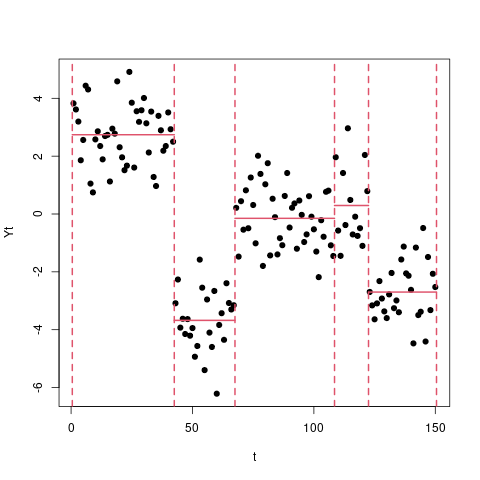
\includegraphics[width=.45\textwidth, trim=0 10 0 10, clip=]{\figcp/FigSeg-HCERES-discrete-seg}
    \end{tabular}
  \end{tabular}
  
  \pause \bigskip
  \paragraph{Aim.}
  Estimate $\tau$ and $\mu$ from $Y$.
  
  \bigskip
  \paragraph{Specificity.}
  $\mu$ is continuous whereas $\tau$ is discrete:
  $\mu \in \Rbb^K$, $\tau \in \llbracket n-1 \rrbracket^{K-1}$.
}

%====================================================================
\frame{\frametitle{Maximum-likelihood inference} 

  \bigskip
  \paragraph{Principle.} 
  For a given number of segments $K$, look for
  $$
  \widehat{\theta} 
  = \argmax_\theta \log p_\theta(Y)
  = \argmin_\theta \sum_{k=1}^K \sum_{t=\tau_{k-1}+1}^{\tau_k} (Y_t - \mu_k)^2
  $$
  where $\theta = (\tau, \mu)$.

  \bigskip \bigskip \pause
  \paragraph{Estimating $\mu$.} 
  For a given $\tau$, we have that
  $$
  \widehat{\mu}_k(\tau) = \argmin_{\mu_k} \sum_{t=\tau_{k-1}+1}^{\tau_k} (Y_t - \mu_k)^2 = \frac1{\tau_k -  \tau_{k-1}} \sum_{t=\tau_{k-1}+1}^{\tau_k} Y_t.
  $$

  \bigskip \bigskip \pause
  \paragraph{Estimating $\tau$.} 
  We are left with the discrete optimization problem
  $$
  \widehat{\tau} 
  = \argmax_\tau \log p_{(\tau, \widehat{\mu}(\tau))}(Y)
  = \argmin_\tau \sum_{k=1}^K \underset{C(\tau_{k-1}+1, \tau_k)}{\underbrace{\sum_{t=\tau_{k-1}+1}^{\tau_k} (Y_t - \widehat{\mu}_k(\tau))^2}}
  $$
}

%====================================================================
\frame{\frametitle{Discrete-time segmentation problem} 

  \begin{itemize}
    \item Consider a cost function $C(t_1, t_2)$ defined for $1 \leq t_1 < t_2 \leq n$;
    \item Define the segmentation space
    $$
    \Tcal_K = \{\tau \in \llbracket n-1 \rrbracket^{K-1}: 
    1 \leq \tau_1 < \dots \tau_{K-1} < n\},
    $$
    observe that 
    $$
    \text{card}(\Tcal) = {{n-1}\choose{K-1}} = \Ocal(n^K);
    $$
    \item Define the contrast $\gamma: \Tcal \mapsto \Rbb$:
    $$
    \gamma(\tau) = \sum_{k=1}^K C(\tau_{k-1}+1, \tau_k), 
    \qquad \text{with } \tau_0 = 0, \tau_K = n.
    $$
    \end{itemize}

  \bigskip \bigskip \pause
  \paragraph{Dynamic programming.}
  The optimal segmentation
  $$
  \widehat{\tau} = \argmin_{\tau \in \Tcal_K} \gamma(\tau)
  $$
  can be recovered in $\Ocal(n^2)$ using a dynamic programming algorithm.
  
}

%====================================================================
%====================================================================
\section{Segmentation in continuous time}
\frame{\frametitle{Outline} \tableofcontents[currentsection]}
%====================================================================
\frame{\frametitle{Maximum-likelihood segmentation} 

  \paragraph{First useful property of Poisson processes:} Independence of disjoint intervals.
  
  \bigskip \bigskip \pause
  \paragraph{(Neg-log-)likelihood.} Denoting
  \begin{itemize}
    \item $\dtau_k$ the length of the $k$-th interval ($= \tau_k - \tau_{k-1}$), 
    \item $\dN_k$ the number of events within the  $k$-th interval ($= N(\tau_k) - N(\tau_{k-1})$):
  \end{itemize}
  \begin{align*}
%     p_{\tau, \lambda}(N) 
%     & = \prod_{k=1}^K  p_{\lambda_k}(N(I_k))
%     = \prod_{k=1}^K  \lambda_k^{\dN_k} \; e^{-\lambda _k \dtau_k}, \\
    - \log p_{\tau, \lambda}(N) 
    & = \sum_{k=1}^K \lambda_k \dtau_k - \dN_k \log \lambda_k, 
%   \qquad \text{where} \quad
%   \left\{ \begin{array}{l}
%             \dN_k = N(\tau_k) - N(\tau_{k-1}), \\
%             \dtau_k = \tau_k - \tau_{k-1}
%           \end{array}\right.
  \end{align*}

  \bigskip \pause
  \paragraph{Additive contrast.} General form = sum over the segments
  $$
  \gamma(\tau, \lambda) = \sum_{k=1}^K C(\dN_k, \dtau_k, \lambda_k)
  $$

  \bigskip \pause
  \paragraph{Optimization problem.} 
  $$
  (\widehat{\tau}, \widehat{\lambda}) = \argmin_{\tau \in \Tcal_K, \lambda \in (\Rbb^+)^K} \; \; \gamma(\tau, \lambda).
  $$
}

%====================================================================
\frame{\frametitle{Minimizing the contrast function} 

  \paragraph{Optimal $\lambda$.}
  Because the contrast is additive, we may define
  $$
  \widehat{\lambda}_k 
  = \widehat{\lambda}_k(\tau)
  = \argmin_{\lambda_k \in \Rbb^+} C(\dN_k, \dtau_k, \lambda_k)
  $$
  e.g. $\widehat{\lambda}_k = \dN_k / \dtau_k$ if $\gamma = -\log p_\theta$.

  \bigskip \bigskip \bigskip \pause
  \paragraph{Optimal $\tau$.}
  We are left with the minimization problem
  $$
  \widehat{\tau} = \argmin_{\tau \in \Tcal_K} \; \; \widehat{\gamma}(\tau), 
  \qquad \text{where} \quad
  \widehat{\gamma}(\tau) = \gamma(\tau, \widehat{\lambda}(\tau))
  $$
  where $\Tcal_K$ is the continuous segmentation space:
  %$\Tcal_K$ is a {\sl continuous set}  :
  $$
  \Tcal_K = \left\{\tau \in [0, 1]^{K+1}: 0 = \tau_0 < \tau_1 \dots < \tau_{K-1} < \tau_K = 1\right\}.
  $$
  
  \bigskip \bigskip \pause
  \paragraph{Main issue:}
  The contrast $\widehat{\gamma}(\tau)$ is \emphase{neither convex nor continuous} wrt $\tau$.

}

%====================================================================
\frame{\frametitle{Shape of the contrast fonction} 

  \begin{tabular}{cc}
    \hspace{-.04\textwidth}
    \begin{tabular}{p{.45\textwidth}}
      \paragraph{Observed $N(t)$:} $n = 10$, \\
      ~ 
    \end{tabular}
    & 
    \hspace{-.05\textwidth}
    \begin{tabular}{p{.55\textwidth}}
      \includegraphics[width=.430\textwidth, height=.25\textheight]{\figcp/FigSegPPP-simul-n10-K1-seed1-Path} \\       
    \end{tabular} 
    \\ \pause
    \hspace{-.04\textwidth}
    \begin{tabular}{p{.45\textwidth}}
      \paragraph{Contrast $\widehat{\gamma}(\tau)$ for $K=3$ segments:}
      $$
      \tau = (\tau_1, \tau_2).
      $$     
     
      \bigskip \bigskip
      One 'block' = \\
      one specific value for the vector \footnote{gray borders come by pair}
      $$
      \dN = (\dN_1, \dN_2, \dN_3)
      $$
      
      \bigskip \bigskip \bigskip ~
    \end{tabular}
    & 
    \hspace{-.05\textwidth}
    \begin{tabular}{p{.55\textwidth}}
      \includegraphics[width=.48\textwidth, trim=0 0 20 50, clip=]{\figcp/FigSegPPP-simul-n10-K1-seed1-Contrast}
    \end{tabular} 
  \end{tabular}

}

%====================================================================
\frame{\frametitle{Partitioning the segmentation space} 

  \paragraph{Partitioning the number of events.} Define
  $
  \Ncal^K = \left\{\nu \in \Nbb^K: \sum_{k=1}^K \nu_k = n\right\}.
  $ \\
  \ra $\nu_k =$ given number of events in segment $k$.

  \bigskip \bigskip \pause
  \begin{tabular}{cc}
    \hspace{-.04\textwidth}
    \begin{tabular}{p{.5\textwidth}}
      \paragraph{Partitioning the segmentation space.} For $\nu \in \Ncal_K$, define
      $$
      \Tcal(\nu) = \left\{\tau \in \Tcal_K: \dN = \nu\right\}.
      $$
      \ra $\Tcal(\nu) =$ set of segmentation satisfying the prescribed $\nu = (\nu_1, \dots \nu_K)$.

      \bigskip
      We have
      $$
      \min_{\tau \in \Tcal_K} \widehat{\gamma}(\tau) 
      = \min_{\nu \in \Ncal^K} \min_{\tau \in \Tcal(\nu)} \widehat{\gamma}(\tau, ).
      $$
    \end{tabular}
    & 
    \hspace{-.05\textwidth}
    \begin{tabular}{p{.5\textwidth}}
      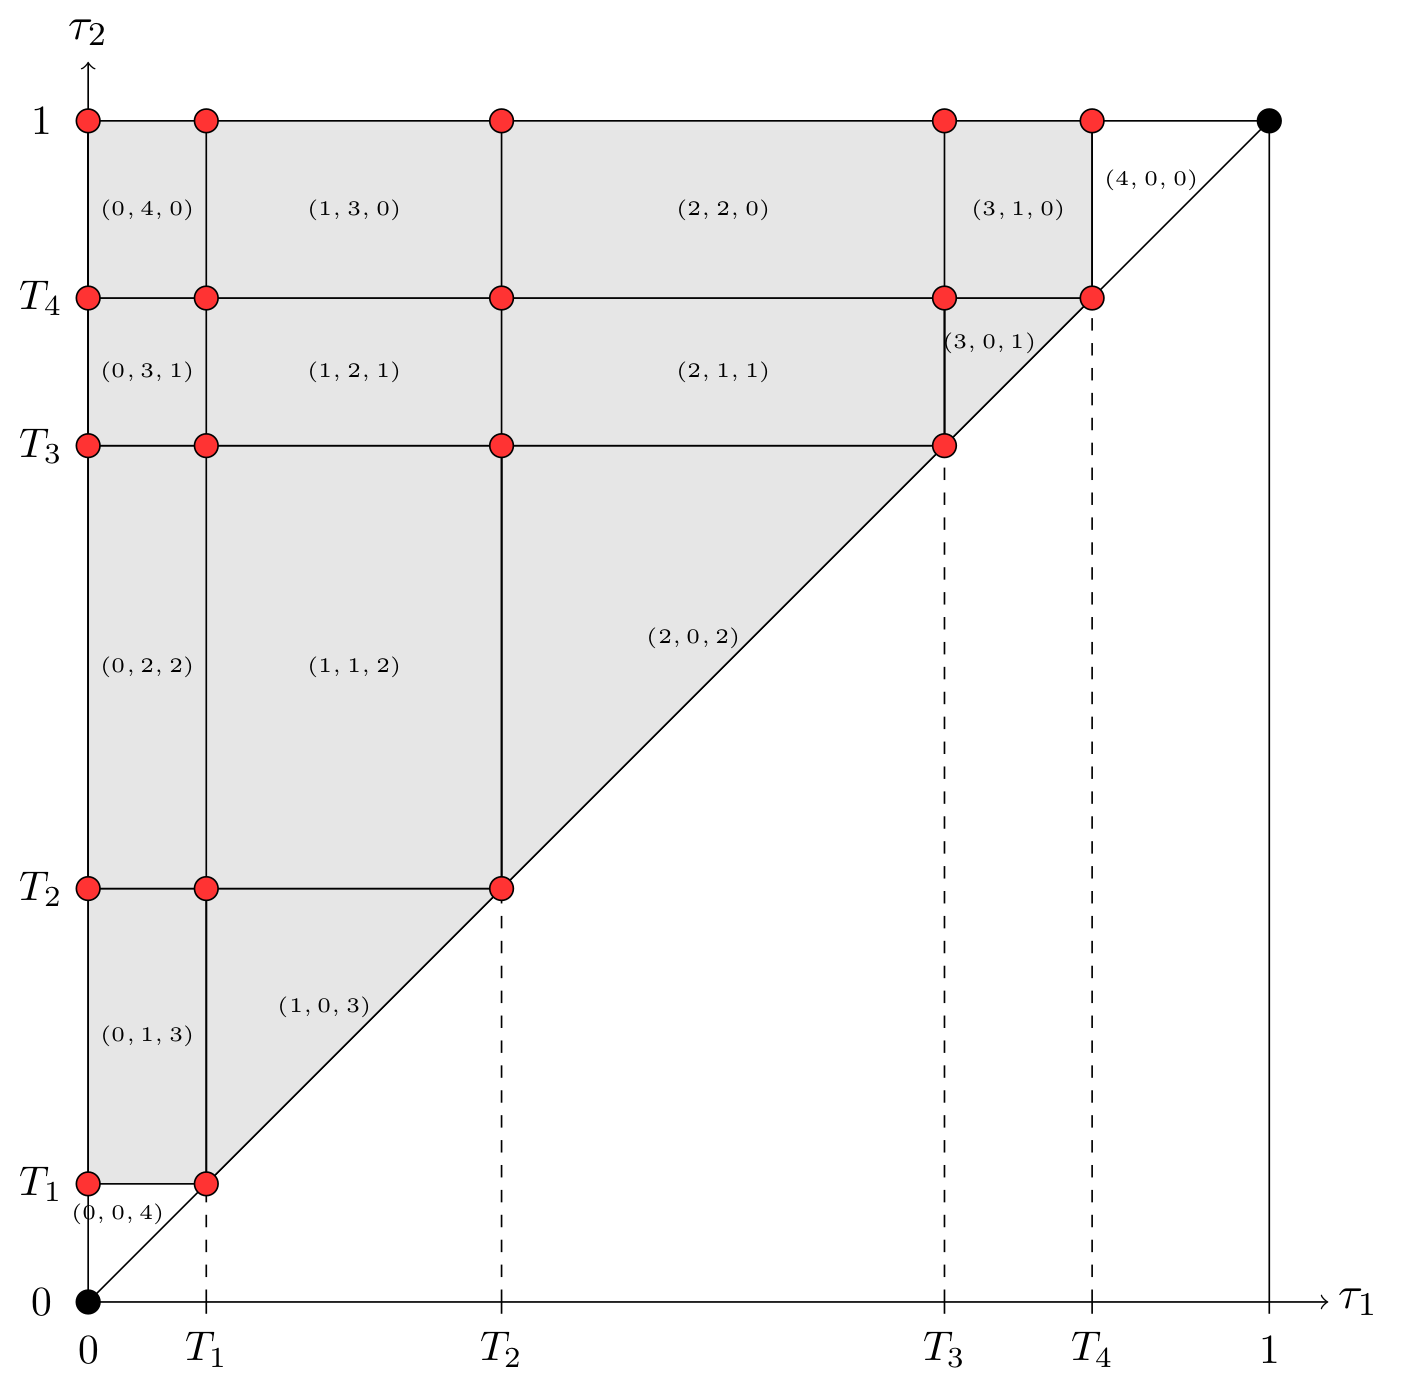
\includegraphics[width=.45\textwidth, trim=0 0 0 0, clip=]{\figcp/DLR23-ArXiv-Fig1}
    \end{tabular}
  \end{tabular}

}

%====================================================================
\frame{\frametitle{Optimal segmentation} 

  \paragraph{Proposition 1.} If $K\leq n$ and 
  \emphase{if $\widehat{\gamma}(\tau)$ is strictly concave wrt $\tau \in \Tcal(\nu)$} for each $\nu \in \Ncal^K$, then
  $$
  \widehat{\tau} = \argmin_{\tau \in \Tcal_K} \widehat{\gamma}(\tau) 
  \subset \{T_1^-, T_1, T_2^-, T_2^-, \dots T_n^-, T_n\}.
  $$

  \bigskip \bigskip \pause  
  \paragraph{Proposition 2.} If each $\widehat{C}(\nu_k, \dtau_k) := C(\nu_k, \dtau_k, \widehat{\lambda}_k)$ is strictly concave wrt $\dtau_k$, then $\widehat{\gamma}(\tau)$ is strictly concave wrt $\tau \in \Tcal(\nu)$.

  \bigskip \bigskip \bigskip \pause
  \paragraph{Consequence.} $\widehat{\tau}$ can be obtained by dynamic programming over the $2n+2$ possible change-points 
  $$
  \Scal = \{0, T_1^-, T_1, T_2^-, T_2, \dots T_n^-, T_n, 1\}
  $$
  with complexity at most $O(n^2)$.
}

%====================================================================
\frame{\frametitle{Admissible contrasts} 

  \paragraph{Poisson contrast.} $\widehat{C}_P(\nu_k, \dtau_k) = \nu_k (1 - \log \nu_k + \log \dtau_k)$ is concave wrt $\dtau$.

  \bigskip \bigskip \bigskip \bigskip \pause
  \paragraph{Poisson-Gamma model.} For each segment $1 \leq k \leq K$:
    $$
    \Lambda_k \text{ iid } \sim \Gam(a, b), \qquad \qquad
    \{N(t)\}_{t \in I_k} \mid \Lambda_k \sim PP(\Lambda_k).
    $$
    
    \bigskip \pause
    Contrast for one segment:
    \begin{align*}
      C_{PG}(\dN_k, \dtau_k) 
      %& = - \log p_{a, b}(\{N(t)\}_{t \in I_k}) \\
      & = \cst - \log \Gamma(a + \dN_k) + (a + \dN_k) \log(b + \dtau_k)
    \end{align*}
    \ra Strictly concave wrt $\dtau_k$.

}

%====================================================================
\frame{\frametitle{Desirable contrast} 

  \paragraph{Remark.} The Poisson contrast $\widehat{C}_P(\nu_k, \dtau_k) = \nu_k (1 - \log \nu_k + \log \dtau_k)$ satisfies
  $$
  \widehat{C}_P(\nu_k = 1, \dtau_k = 0) = -\infty.
  $$
  \begin{itemize}
    \setlength{\itemsep}{1.1\baselineskip}
    \item The optimal solution will involve segments with null length and containing only one event. 
    \item 'Undesirable' contrast.
  \end{itemize}


  \bigskip \bigskip \bigskip \pause
  \paragraph{Poisson-Gamma contrast.} $C_{PG}(\nu_k, \dtau_k) = - \log \Gamma(a + \nu_k) + (a + \nu_k) \log(b + \dtau_k)$. \\
  ~
  \begin{itemize}
    \setlength{\itemsep}{1.1\baselineskip}
    \item Satisfies the concavity property (\ra admissible), 
    \item but avoids segments with null length (\ra desirable).
  \end{itemize}
  
}

%====================================================================
%====================================================================
\section{Model selection}
\frame{\frametitle{Outline} \tableofcontents[currentsection]}
%====================================================================
\frame{\frametitle{Model selection} 

  \paragraph{Second useful property of Poisson processes:} Thining. ~ \\
  \begin{tabular}{cc}
    \hspace{-.04\textwidth}
    \begin{tabular}{p{.5\textwidth}}
      \begin{itemize}
        \setlength{\itemsep}{1.1\baselineskip}
        \item $\{N(t)\} \sim PP(\lambda(t))$
        \item \textcolor{blue}{Sample event times} (with prob. $f$) 
        \item \textcolor{red}{Store the remaining events}
      \end{itemize}
    \end{tabular}
    & 
    \hspace{-.15\textwidth}
    \begin{tabular}{p{.4\textwidth}}
      \begin{overprint}
        \onslide<1>
        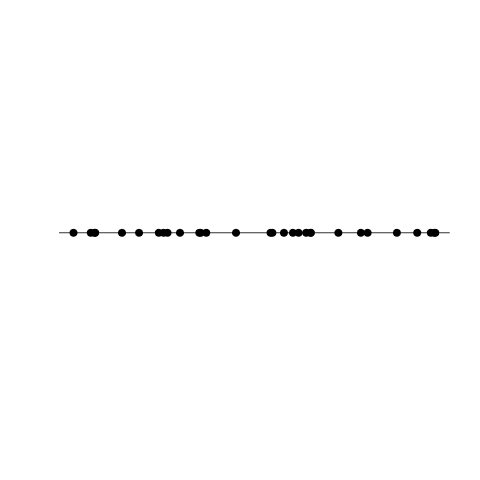
\includegraphics[width=.5\textwidth, trim=0 225 0 225, clip=]{\figcp/FigSegPP-ThiningOriginal.png}
        \onslide<2->
        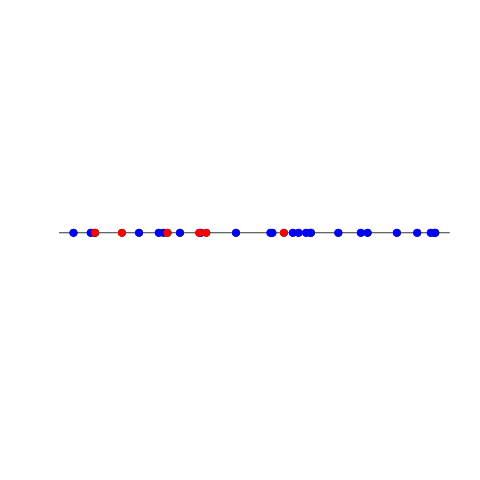
\includegraphics[width=.5\textwidth, trim=0 225 0 225, clip=]{\figcp/FigSegPP-ThiningSampling.png}
      \end{overprint}
    \end{tabular}
  \end{tabular}
  \pause
  $$
  \textcolor{blue}{\{N^L(t)\}} \sim PP(f\lambda(t)), \qquad
  \textcolor{red}{\{N^T(t)\}} \sim PP((1-f)\lambda(t)), \qquad
  {\{N^L(t)\}} \perp {\{N^T(t)\}}
  $$
  
  \bigskip \bigskip \pause
  \paragraph{Consequence.} If $\{N(t)\}_{0 \leq t \leq 1} \sim PP(\lambda(t))$, with $\lambda(t)$ piecewise constant with change-points $\tau = (\tau_k)$ and intensities $\lambda = (\lambda_k)$, then \\ ~ \pause
  \begin{itemize}
    \setlength{\itemsep}{1.1\baselineskip}
    \item $\textcolor{blue}{\lambda^L(t)}$ piecewise constant with change-points $(\textcolor{blue}{\tau_k})$ and intensities $(\textcolor{blue}{f \lambda_k})$, 
    \item $\textcolor{red}{\lambda^T(t)}$ piecewise constant with change-points $(\textcolor{red}{\tau_k})$ and intensities $(\textcolor{red}{(1-f) \lambda_k})$, 
    \item $\{N^L(t)\} \perp \{N^T(t)\}$.
  \end{itemize}
}

%====================================================================
\frame{\frametitle{Cross validation} 

  Sampling event times provides two independent Poisson processes with \emphase{same change-points}.
  
  \bigskip \bigskip \pause
  \paragraph{Cross-validation procedure.} For $1 \leq K \leq K_{\max}$, \\ ~
  \begin{itemize}
   \item Repeat for $1 \leq m \leq M$ : \\
      \medskip
      1 -- Sample the event times to form $\textcolor{blue}{\{N^{L, m}(t)\}}$ (learn) and $\textcolor{red}{\{N^{T, m}(t)\}}$ (test), \\
      \medskip
      2 -- Estimate $\widehat{\tau}^{L, m}$ and $\widehat{\lambda}^{L, m}$ from $\textcolor{blue}{\{N^{L, m}(t)\}}$, \\
      \medskip
      3 -- Compute the contrast $\displaystyle{\gamma_K^{T, m} = \gamma\left(\textcolor{red}{\{N^T(t)\}}; \widehat{\tau}^{L, m}, \textcolor{red}{\frac{1-f}{f}}\widehat{\lambda}^{L, m}\right)}$.
    \bigskip
    \item \pause Compute
    $$
    \overline{\gamma}_K = \frac1M \sum_{m=1}^M \gamma_K^{T, m}
    $$
    \medskip
    \item \pause Select
    $$
    \widehat{K} = \argmin_K \overline{\gamma}_K
    $$
  \end{itemize}
}

%====================================================================
%====================================================================
\section{Illustrations}
\frame{\frametitle{Outline} \tableofcontents[currentsection]}
%====================================================================
\frame{\frametitle{Practical implementation.} 
%====================================================================

  \paragraph{Contrasts.} During the CV process, we use
  \begin{itemize}
    \item a sampling rate of $f = 4/5$, 
    \item the Poisson-Gamma contrast $\gamma_{PG}$ for the learning step and
    \item the Poisson contrast $\gamma_P$ for the test step.
  \end{itemize}
  
  \bigskip \bigskip \pause
  \paragraph{Hyper-parameters.} For an observed path $\{N(t)\}_{0 \leq t \leq 1}$ with $n = N(1)$ events, we use 
  $$
  a = 1, \qquad b = 1/n
  $$
  to fit the observed total number of events.
  
  \bigskip \bigskip \bigskip \pause
  \paragraph{R package {\tt CptPointProcess}} available on \url{github.com/Elebarbier/CptPointProcess}.
}

%====================================================================
\frame{\frametitle{Some simulations} 

  \bigskip
  \paragraph{Simulation setting.} $K = 6$ segments with varying length. Tuning parameters:
  \begin{itemize}
    \item $\overline{\lambda}$ average intensity (\ra total number of events), 
    \item $\lambda_R =$ height of the steps (\ra contrast between segments).
  \end{itemize}

  \bigskip \bigskip \pause
  \paragraph{Intensity function $\lambda(t)$.} $\overline{\lambda} = 100$, $\lambda_R = 1, 3, 8$.
  $$
  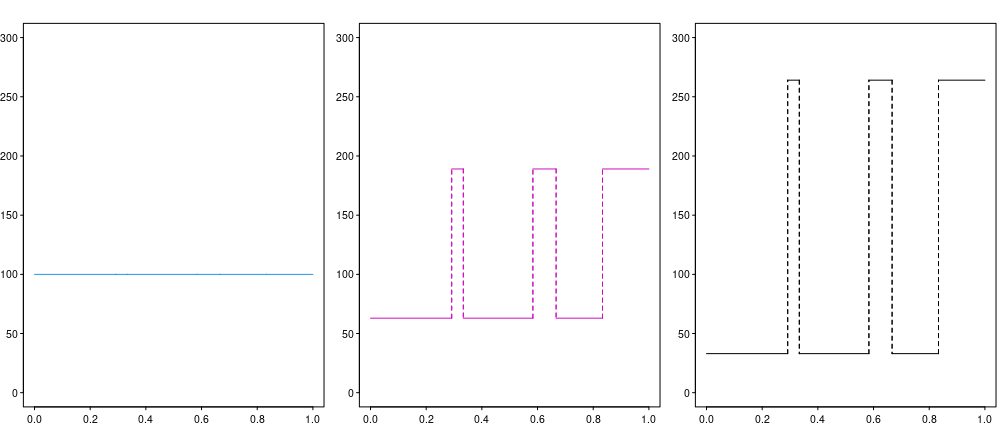
\includegraphics[width=.6\textwidth, trim=0 10 0 10, clip=]{\figcp/DLR23-ArXiv-Fig2}
  $$
  
}

%====================================================================
\frame{\frametitle{Some simulations} 

  \paragraph{Estimation.} Choose $K$ via CV, then refit the parameters to the whole dataset.

  \bigskip \bigskip \pause
  \paragraph{Results.}  $x$-axis = $\lambda_R$, color = $\overline{\lambda}$
  \bigskip
  \begin{tabular}{ccc}
    Model selection & 
    Change-point location & 
    Cumulated intensity  \\
    $\widehat{K}$ & 
    Haussdorf$(\widehat{\tau}, \tau^*)$ & 
    $\ell_2(\widehat{\Lambda}, \Lambda^*)$ \\
    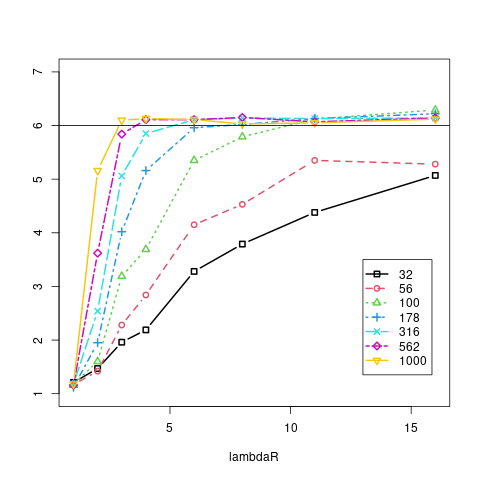
\includegraphics[width=.3\textwidth, trim=10 10 20 20, clip=]{\figcp/DLR23-ArXiv-Fig3}
    &
    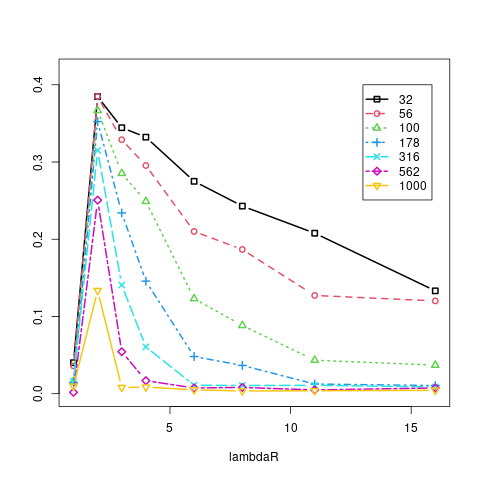
\includegraphics[width=.3\textwidth, trim=10 10 20 20, clip=]{\figcp/DLR23-ArXiv-Fig4a}
    &
    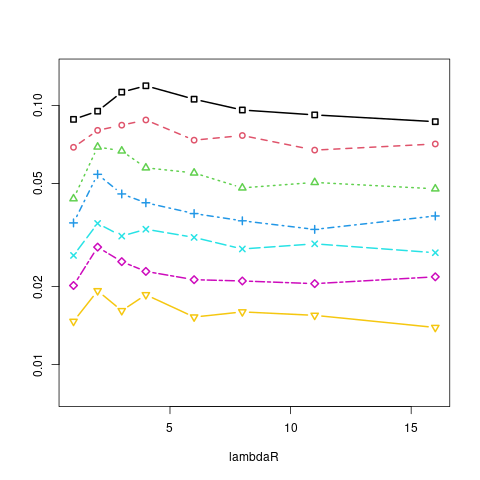
\includegraphics[width=.3\textwidth, trim=10 10 20 20, clip=]{\figcp/DLR23-ArXiv-Fig4b}    
  \end{tabular}

}

%====================================================================
\frame{\frametitle{Kilauea eruptions} 

  \paragraph{$n = 63$ eruptions} reported between the mid 18th and the late 20th century. \\ ~
  
  $$
  \begin{tabular}{cc}
    Model selection via CV &
    Resulting segmentation \\
    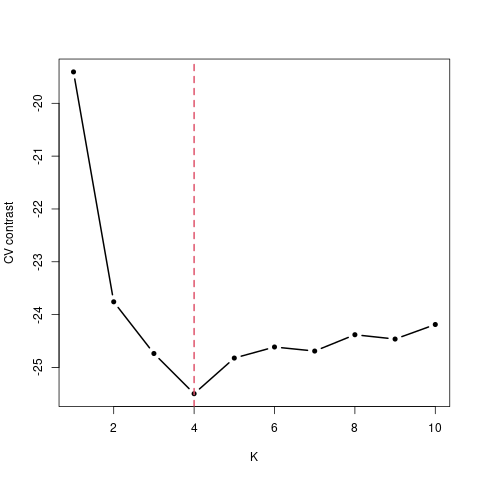
\includegraphics[width=.35\textwidth, trim=0 10 10 10, clip=]{\figcp/DLR23-ArXiv-Fig5a}
    & 
    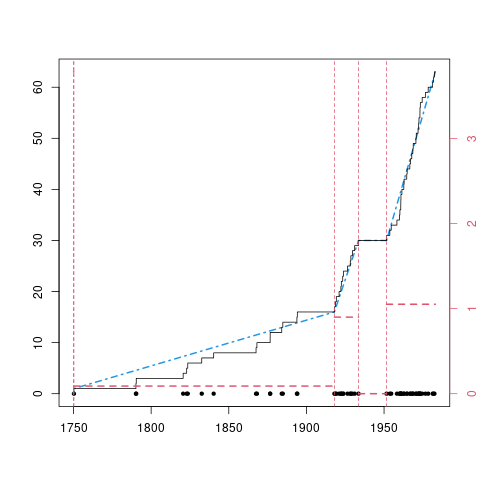
\includegraphics[width=.35\textwidth, trim=0 10 0 10, clip=]{\figcp/DLR23-ArXiv-Fig6a}
  \end{tabular}
  $$
}

%====================================================================
%====================================================================
\section{Extensions \& future works}
\frame{\frametitle{Outline} \tableofcontents[currentsection]}
%====================================================================
\frame{\frametitle{Marked-Poisson processes} 

  \paragraph{Marked Poisson Process.}
  \begin{itemize}
    \setlength{\itemsep}{1.1\baselineskip}
    \item $\{Y(t)\}_{0 \leq t \leq 1} \sim MPP(\lambda(t), \mu(t))$:
    $$
    \{N(t)\}_{0 \leq t \leq 1} \sim PP(\lambda(t)), \qquad
    \text{at each $T_i$:} \quad X_i \sim \Fcal(\mu(T_i))
    $$
    \item Volcanos: mark = eruption duration.
    \item Bat cries: mark = bat species or cry duration.
  \end{itemize}

  \bigskip \bigskip \pause
  \paragraph{Proposed method.}
  \begin{itemize}
    \setlength{\itemsep}{1.1\baselineskip}
    \item Works the same way, provided that concavity holds.
    \item Poisson-Gamma events + Exponential-Gamma durations is both admissible and desirable.
  \end{itemize}

}

%====================================================================
\frame{\frametitle{Marked Poisson process: Etna eruptions} 

  \paragraph{Count and marks:} Events = eruptions, marks = duration of each eruption.
  
  \bigskip \bigskip 
  \paragraph{Model.} 
  \begin{itemize}
    \item Piecewise-constant intensity Poisson process for the events
    \item Exponential distribution (with segment specific parm.) for the durations
  \end{itemize}
  
  \bigskip \bigskip \pause
  \paragraph{CV for the selection of $K$.} 
  $$
  \begin{tabular}{cc}
    Poisson & Marked Poisson \\
    \includegraphics[width=.4\textwidth, trim=0 10 10 30, clip=]{\figcp/DLR23-ArXiv-Fig7a}    
    &
    \includegraphics[width=.4\textwidth, trim=0 10 10 30, clip=]{\figcp/DLR23-ArXiv-Fig7b} \\
%     Events & Events \qquad \qquad \qquad \qquad \qquad Marks \\
%     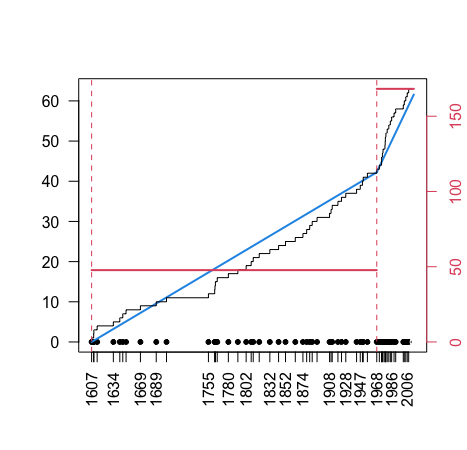
\includegraphics[width=.3\textwidth, height=.325\textheight, trim=0 35 10 50, clip=]{\figcp/DLR23-ArXiv-Fig8a}
%     &
%     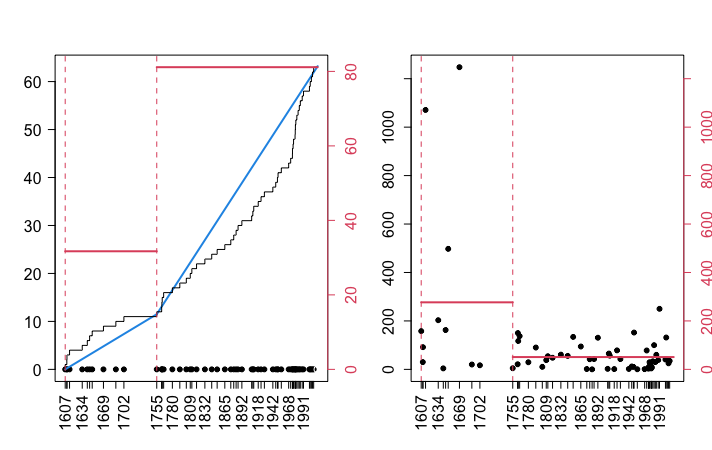
\includegraphics[width=.6\textwidth, height=.3\textheight, trim=0 10 10 50, clip=]{\figcp/DLR23-ArXiv-Fig8bc}    
  \end{tabular}
  $$

}

%====================================================================
\frame{\frametitle{Marked Poisson process: Etna eruptions} 

  $$
  \begin{tabular}{c|c}
    Poisson ($\widehat{K} = 2$) & Marked Poisson ($\widehat{K} = 2$) \\
%     \includegraphics[width=.25\textwidth, height=.3\textheight, trim=0 10 10 30, clip=]{\figcp/DLR23-ArXiv-Fig7a}    
%     &
%     \includegraphics[width=.25\textwidth, height=.3\textheight, trim=0 10 10 30, clip=]{\figcp/DLR23-ArXiv-Fig7b} \\
    Events & Events \qquad \qquad \qquad \qquad \qquad Marks \\
    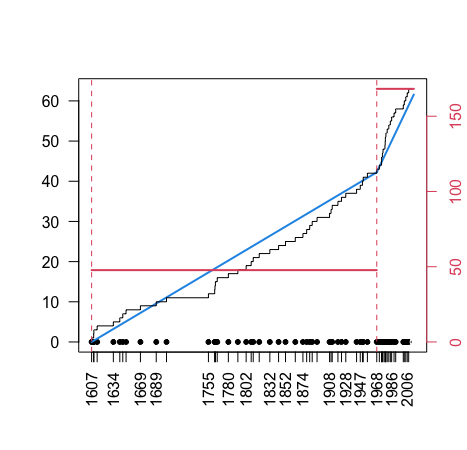
\includegraphics[width=.3\textwidth, height=.325\textheight, trim=0 35 10 50, clip=]{\figcp/DLR23-ArXiv-Fig8a}
    &
    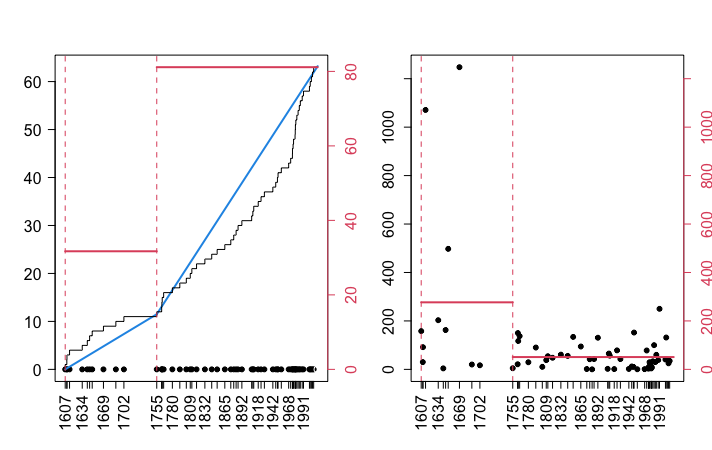
\includegraphics[width=.6\textwidth, height=.3\textheight, trim=0 10 10 50, clip=]{\figcp/DLR23-ArXiv-Fig8bc} \\
    \hline
    \pause
    & Marked Poisson ($K = 3$) \\
    & Events \qquad \qquad \qquad \qquad \qquad Marks \\
    &  
    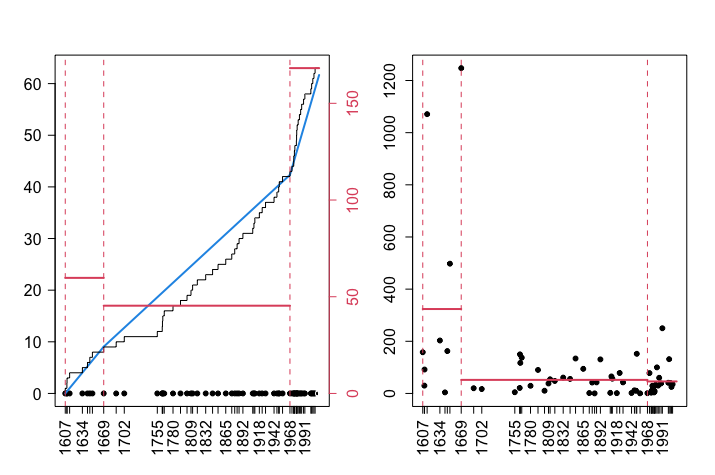
\includegraphics[width=.6\textwidth, height=.3\textheight, trim=0 35 10 10, clip=]{\figcp/DLR23-ArXiv-Fig9}    
  \end{tabular}
  $$

}

%====================================================================
\frame{\frametitle{Model selection} 

  \paragraph{Poisson process: Mauna Loa eruptions.} $n = 40$
  $$
  \begin{tabular}{ccc}
    $K = 2$ & $K = 3$ & $K = 4$ \\
    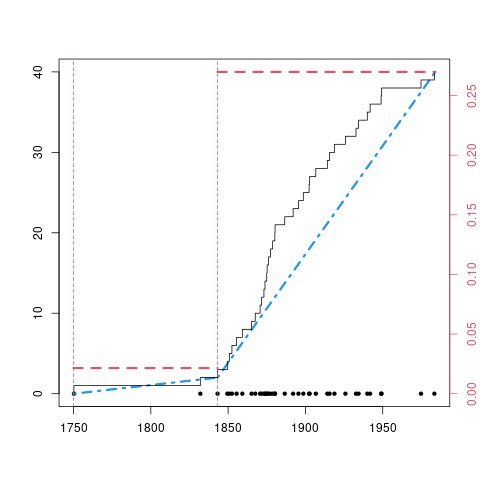
\includegraphics[width=.25\textwidth, trim=0 35 10 50, clip=]{\figcp/DLR23-ArXiv-Fig10_}    
    &
    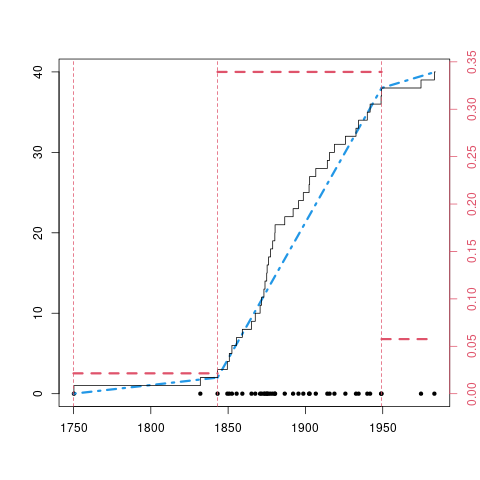
\includegraphics[width=.25\textwidth, trim=0 35 10 50, clip=]{\figcp/DLR23-ArXiv-Fig10a}    
    &
    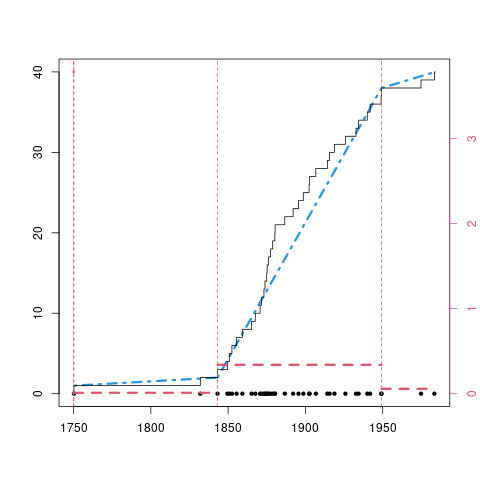
\includegraphics[width=.25\textwidth, trim=0 35 10 50, clip=]{\figcp/DLR23-ArXiv-Fig10b}    
    \\ ~ \\
    $K = 5$ & $K = 6$ \\
    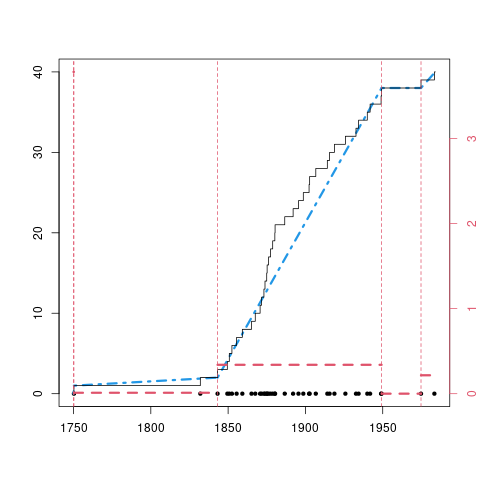
\includegraphics[width=.25\textwidth, trim=0 35 10 50, clip=]{\figcp/DLR23-ArXiv-Fig10c}    
    &
    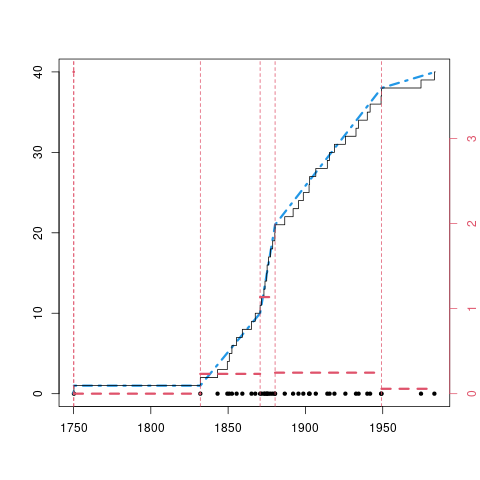
\includegraphics[width=.25\textwidth, trim=0 35 10 50, clip=]{\figcp/DLR23-ArXiv-Fig10d}    
  \end{tabular}
  $$

}

%====================================================================
\frame{\frametitle{Model selection} 

  \paragraph{Choice of the fraction $f$ for cross-validation.} 
  Proposed $f = 4/5$ \\
  
  \bigskip
  Synthetic data: $\overline{\lambda} = 100$ and $\lambda_R=8$
  $$
  \begin{array}{ccc}
    \widehat{K} & d(\widehat{\tau}, \tau) & \ell_2(\widehat{\Lambda}, \Lambda) \\
    \includegraphics[width=.3\textwidth, trim=10 10 10 50, clip=]{\figDLR/Kcv-V} & 
    \includegraphics[width=.3\textwidth, trim=10 10 10 50, clip=]{\figDLR/Hausdorff-V} & 
    \includegraphics[width=.3\textwidth, trim=10 10 10 50, clip=]{\figDLR/relL2cum-V}     
  \end{array}
  $$

  \bigskip \pause
  \paragraph{Ongoing work.}
  \begin{itemize}
    \item Need for an alternative criterium, e.g. BIC
    \item Consistency of the estimated change-points 
  \end{itemize}
  
  }

%====================================================================
%====================================================================
\section{Future works}
\frame{\frametitle{Outline} \tableofcontents[currentsection]}
%====================================================================
\frame{\frametitle{Future works} 

  \paragraph{Segmentation-clustering.}
  \begin{itemize}
    \setlength{\itemsep}{1.1\baselineskip}
    \item Each segment belongs to a class $1 \leq q \leq Q$ (with probability $\pi_q$ and intensity $\lambda_k = \ell_q$), 
    \item Combination of EM and DP algorithms \refer{PRL07}, 
    \item Bat cries: Class = animal behaviour (hunt, transit, ...)
  \end{itemize}

  \bigskip \bigskip \pause
  \paragraph{Hawkes process.}
  \begin{itemize}
    \setlength{\itemsep}{1.1\baselineskip}
    \item Accounts for sel excication (or inhibition), but yields non-additive contrasts
    \item Markovian reformulation of the discrete-time approximation, with exponential kernel
    \item Segmentation-clustering doable via $\simeq$ classical hidden Markov modeling
  \end{itemize}
}

%====================================================================
\frame[allowframebreaks]{ \frametitle{References}
  {
   \small
   \nocite{DLR23}
   \bibliography{/home/robin/Biblio/BibGene}
   \bibliographystyle{alpha}
  }
}

%====================================================================
\backupbegin
%====================================================================

%====================================================================
\frame{\frametitle{Dynamic programming} 

  \paragraph{Belman's principle.}
  All sub-paths of the optimal path must be optimal themselves.
  
  \pause \bigskip 
  \paragraph{Dynamic programming algorithm \refer{AuL89}.}
  \begin{enumerate}
    \item For each $m \in \llbracket n\rrbracket$, compute (in $\Ocal(m)$)
    $$
    t_1(m) = \argmin_{1 \leq t < m} C(1, t) + C(t+1, m), 
    \qquad
    S_2(m) = \min_{1 \leq t < m}();
    $$
    \item Then, for each $k = 3 \dots K$ and each $m \in \llbracket n\rrbracket$, compute  (in $\Ocal(m)$)
    $$
    t_{k-1}(m) = \argmin_{k-1 \leq t < m} S_{k-1}(1, t) + C(t+1, m), 
    \qquad
    S_k(m) = \min_{k-1 \leq t < m} (). 
    $$
  \end{enumerate}
  
  \pause \bigskip  \bigskip 
  \paragraph{Solution.}
  After $\Ocal(Kn^2)$ operations:
  $$
  \min_{\tau \in \Tcal_K} \gamma(\tau) = S_K(n), 
  $$
  and 
  $$
  \widehat{\tau}_{K-1} = t_{K-1}(n), 
  \qquad
  \widehat{\tau}_{k-1} = t_{K-1}(\widehat{\tau}_k).
  $$
  

}

%====================================================================
\frame{\frametitle{Appendix} 

  \paragraph{Number of elements in the partition of the segmentation space.}
  $$
  |\Ncal_K| = \sum_{h=\lfloor (K-1)/2\rfloor}^K {{n-1}\choose{h-1}} {{h+1}\choose{K-h}}
  $$

  \bigskip \bigskip \bigskip \pause
  \paragraph{Simulations: Shape of the intensity function $\lambda(t)$.} $K=6$, $\overline{\lambda} = 100$, $\lambda_R = 1, 3, 8$.
  $$
  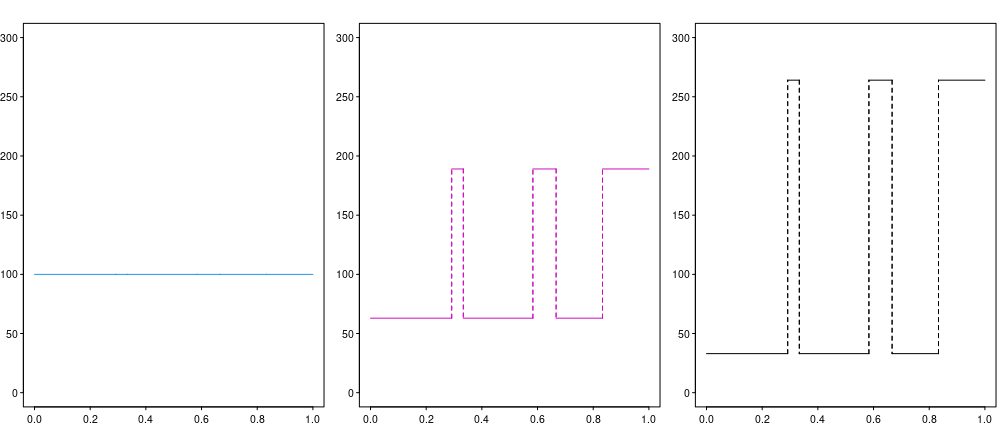
\includegraphics[width=.6\textwidth, trim=0 10 0 10, clip=]{\figcp/DLR23-ArXiv-Fig2}
  $$

}

%====================================================================
\frame{\frametitle{Choice of the hyper-parameters $(a, b)$} 

  Sticking to $a/b = n$ ($\overline{\lambda} = 100$ and $\lambda_R=8$) :

  \bigskip \bigskip 
  \begin{tabular}{ccc}
    $\widehat{K}$ & $d(\widehat{\tau}, \tau)$ & $\ell_2(\widehat{\Lambda}, \Lambda)$ \\
    \includegraphics[width=.3\textwidth, trim=10 10 10 10 50, clip=]{\figDLR/Kcv-a} & 
    \includegraphics[width=.3\textwidth, trim=10 10 10 10 50, clip=]{\figDLR/Hausdorff-a} & 
    \includegraphics[width=.3\textwidth, trim=10 10 10 10 50, clip=]{\figDLR/relL2cum-a}     
  \end{tabular}

}

%====================================================================
\frame{\frametitle{Segmentation in a Hawkes process} 

  \paragraph{Modeling.} Many counting processes display a self-exciting behavior (events generate --~or prevent~-- new events), which the Poisson process does not account for.
  
  \pause \bigskip \bigskip
  \paragraph{Hawkes process.} Counting process $N(t)$ with intensity conditional on the past events:
  $$
  \lambda(t) 
  = m + \int_0^t h(t-s) d N(s) 
  = m + \sum_{i: T_i < t} h(t -T_i).
  $$
  \begin{itemize}
    \item $m =$ baseline intensity,
    \item $h =$ kernel, e.g. exponential: $h(u) = a e^{-bu}$.
  \end{itemize}

  \pause \bigskip \bigskip 
  \paragraph{Change point detection in the baseline.} Change-points $0 < \tau_1 < \dots < \tau_{K-1} < 1$:
  $$
  \lambda(t) 
  = m_k + \sum_{i: T_i < t} h(t -T_i), 
  \qquad \text{if} \quad
  \tau_{k-1} < t \leq \tau_k.
  $$

}

%====================================================================
\frame{\frametitle{Segmentation in a Hawkes process: Discrete time} 

  \paragraph{Non-additive contrast.} Disjoint time segments are not independent, so  classical contrasts (e.g. negative log-likelihood, \dots) are not additive anymore.

  \pause \bigskip \bigskip 
  \paragraph{Discrete time Hawkes process.} Consider discrete times $t_i = i/n$ and define
  $$
  Y_i \sim \Pcal\left(\mu + \sum_{j \geq 1} \alpha \beta^j Y_{i-j}\right)
  $$
  (taking $\mu = m/n$,  $\beta = e^{-b/n}$).

  \pause \bigskip \bigskip 
  \paragraph{Makovian reformulation.} 
  \begin{itemize}
    \setlength{\itemsep}{1\baselineskip}  
    \item $\{Y_i\}_{i \geq 1}$ is not a Markov chain,
    \item but, defining $U_1 = 0$ and
    $$
    U_i = \beta \left(\alpha Y_{i-1} + U_{i-1}\right),
    \qquad \text{for} \quad i \geq 1,
    $$
    $\{(Y_i, U_i)\}_{i \geq 1}$ is a Markov chain.
  \end{itemize}
  
}

%====================================================================
\frame{\frametitle{Segmentation and classification in a Hawkes process: Discrete time} 

  \paragraph{Hidden Markov models (HMM)} provide a convenient framework for segmentation and classification.
  
  \pause \bigskip \bigskip
  \paragraph{Discrete time Hawkes HMM.}   
  \begin{itemize}
    \setlength{\itemsep}{1\baselineskip}  
    \item Hidden path: $\{Z_i\}_{i \leq 1} =$ homogeneous Markov chain, with transition matrix $\pi$, 
    \item 'Observed path': for $i \geq 1$, set $U_1 = 0$ and
    $$
    Y_i \sim \Pcal\left(\mu_{Z_i} + \sum_{j \geq 1} \alpha \beta^j Y_{i-j}\right), 
    \qquad \qquad 
    U_i = \alpha Y_{i-1} + \beta U_{i-1}.
    $$
  \end{itemize}

  \pause \bigskip
  \paragraph{Inference.} Regular EM algorithm for HMM.


  \pause \bigskip \bigskip
  \paragraph{Extensions.}
  \begin{itemize}
    \item Multivariate (discrete time) Hawkes process.
    \item Applications: neuro-sciences, ecology.
  \end{itemize}

}

%====================================================================
\frame{\frametitle{HMM for discrete time Hawkes process} 

  \renewcommand{\nodesize}{2em}
  \renewcommand{\edgeunit}{3*\nodesize}

  \paragraph{Graphical model.} 
  
  \begin{center}
  \begin{tikzpicture}
\node[] (Zt_2) at (-\edgeunit, \edgeunit) {}; 
\node[] (Zt_1) at (0, \edgeunit) {$Z_{i-1}$}; 
\node[] (Zt) at (\edgeunit, \edgeunit) {$Z_{i}$}; 
\node[] (Zt1) at (2*\edgeunit, \edgeunit) {$Z_{i+1}$}; 
\node[] (Zt2) at (3*\edgeunit, \edgeunit) {}; 
\node[] (Ut_1) at (-0.5*\edgeunit, 0.5*\edgeunit) {$U_{i-1}$}; 
\node[] (Ut) at (0.5*\edgeunit, 0.5*\edgeunit) {$U_{i}$}; 
\node[] (Ut1) at (1.5*\edgeunit, 0.5*\edgeunit) {$U_{i+1}$}; 
\node[] (Ut2) at (2.5*\edgeunit, 0.5*\edgeunit) {$U_{i+2}$}; 
\node[] (Ut3) at (3.5*\edgeunit, 0.5*\edgeunit) {}; 
\node[] (Yt_2) at (-\edgeunit, 0) {}; 
\node[] (Yt_1) at (0, 0) {$Y_{i-1}$}; 
\node[] (Yt) at (\edgeunit, 0) {$Y_{i}$}; 
\node[] (Yt1) at (2*\edgeunit, 0) {$Y_{i+1}$}; 
\node[] (Yt2) at (3*\edgeunit, 0) {}; 

\draw[->,dashed] (Zt_2) -- (Zt_1); \draw[->] (Zt_1) -- (Zt); \draw[->] (Zt) -- (Zt1); \draw[->,dashed] (Zt1) -- (Zt2);
\draw[->] (Zt_1) -- (Yt_1); \draw[->] (Zt) -- (Yt); \draw[->] (Zt1) -- (Yt1);
\draw[->] (Ut_1) -- (Yt_1); \draw[->] (Ut) -- (Yt); \draw[->] (Ut1) -- (Yt1);
\draw[->] (Ut_1) -- (Ut); \draw[->] (Ut) -- (Ut1); \draw[->] (Ut1) -- (Ut2); \draw[->,dashed] (Ut2) -- (Ut3);
\draw[->,dashed] (Yt_2) -- (Ut_1); \draw[->] (Yt_1) -- (Ut); \draw[->] (Yt) -- (Ut1); \draw[->] (Yt1) -- (Ut2);
\end{tikzpicture}


  \end{center}
}

%====================================================================
\backupend
%====================================================================

%====================================================================
%====================================================================
\end{document}
%====================================================================
%====================================================================
  
  \begin{tabular}{cc}
    \hspace{-.04\textwidth}
    \begin{tabular}{p{.5\textwidth}}
    \end{tabular}
    & 
    \hspace{-.02\textwidth}
    \begin{tabular}{p{.5\textwidth}}
    \end{tabular}
  \end{tabular}


